\documentclass[11pt, english]{article}
%\usepackage[latin1]{inputenc}
\usepackage[T1]{fontenc}
\usepackage[utf8]{inputenc}
\usepackage[english]{babel}   % S P R A A K
% \usepackage{graphicx}    % postscript graphics
\usepackage{amssymb, amsmath, amsthm, amssymb} % symboler, osv
\usepackage{mathrsfs}
\usepackage{url}
\usepackage{thmtools}
\usepackage{enumerate}  % lister $  
\usepackage{float}
\usepackage{tikz}
\usepackage{tikz-cd}
\usetikzlibrary{calc}
%\usepackage{tikz-3dplot}
\usepackage{subcaption}
\usepackage[all]{xy}   % for comm.diagram
\usepackage{wrapfig} % for float right
\usepackage{hyperref}
\usepackage{mystyle} % stilfilen      

%\usepackage[a5paper,margin=0.5in]{geometry}


\begin{document}
\title{Summary}
\author{Fredrik Meyer}
\maketitle 

\section{Dimension of some cohomology groups}

\begin{tabular}{ l || c | r | r | r | r | r | c  }
 Group & 0 & 1 & 2 & 3 & 4 & 5 & Euler-characteristic \\
\hline
$H^i(X, \Omega_{\PP^{12}} \otimes \OO_X)$ & 0 & 1 & 0 & 167 & 0 & 0 & -168\\
$H^i(Y, I_Y/I_Y^2)$ & 0 & 36 & 0 & 12 & 2 & 0 & -46 \\
$H^i(Y, \Omega_Y)$ & 0 & 1  & 12 & 2 & 0  & 0 & -9
\end{tabular}


\section{The singular locus of $Y$}

By computing in each chart and taking closures, it can be computed that the singular locus of $Y$ is of dimension $1$, and consists of the union of projective lines:

\section{Deformations of $dP_6$}

We will need some results about deformations of the cone over $dP_6$. 

Recall that $dP_6$ is the toric variety whose associated polytope is the hexagon:

\begin{center}
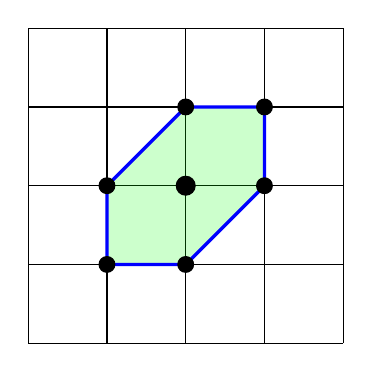
\begin{tikzpicture}
  \draw (0, 0) grid (4, 4);  

\draw [very thick, color=blue, fill=green, fill opacity=0.2]
(1,1) -- (2,1) -- (3,2) -- (3,3) -- (2,3) -- (1,2) -- cycle;

\draw [fill=black]  (1, 1) circle (0.1);
\draw [fill=black]  (2, 1) circle (0.1);
\draw [fill=black]  (3, 2) circle (0.1);
\draw [fill=black]  (3, 3) circle (0.1);
\draw [fill=black]  (2, 3) circle (0.1);
\draw [fill=black]  (1, 2) circle (0.1);
\draw [fill=black]  (2, 2) circle (0.12);
\end{tikzpicture}
\end{center}

This induces an embedding into $\PP^6$. Let $\PP^6$ have coordinates $y_0,x_1..x_6$ (corresponding to the center and the vertices, respectively). Then the ideal of $dP_6$ inside $\PP^6$ is given by the $2 \times 2$-minors of the matrix
\begin{equation}
\label{eqdp6}
\begin{vmatrix}
x_1 & y_0 & x_6 \\
x_2 & x_3 & y_0 \\
y_0 & x_4 & x_5
\end{vmatrix} \leq 1.
\end{equation}

The $\Z_6$-symmetry is visible by permuting columns and rows. Since $dP_6$ is smooth, the only singularity of its affine cone, $C(dP_6)$, is the origin. One can compute that $T^1(C(dP_6))=3$, and that the versal base space splits into two components. Up to a change of variable, the two deformations of the affine cone is given by
\[
\begin{vmatrix}
x_1 & y_0+t_3 & x_6 \\
x_2 & x_3 & y_0+t_3 \\
y_0+t_3 & x_4 & x_5
\end{vmatrix} \leq 1.
\]
and 
\[
\begin{vmatrix}
x_1 & y_0-t_2+t_1 & x_6 \\
x_2 & x_3 & y_0+t_1+t_2 \\
y_0-t_2-t_1 & x_4 & x_5
\end{vmatrix} \leq 1.
\]

Note that by the form of the equations \eqref{eqdp6}, there is a factorization.
\[
\xymatrix{
dP_6  \ar@{^(->}[r] \ar@{^(->}[dr]& \PP^2 \times \PP^2 \ar@{^(->}[d] \\
& \PP^8
}
\]
The two deformations behave differently with resepct to this factorization. The first deformation is induced by a deformation of $C(\PP^2 \times \PP^2)$, leaving the ideal fixed. The other deformation is obtained by also deforming the ideal.



\end{document}
